%%=============================================================================
%% Onderzoek
%%=============================================================================

\chapter{\IfLanguageName{dutch}{Onderzoek}{Study}}
\label{ch:onderzoek}



In this study there will be a comparison between the GNFS algorithm on a classical computer and Shor's algorithm on a quantum computer.
Section \ref{sec:Other algorithms} will discuss some other algorithms that can show the benefits of quantum computing in the industry. To conclude there will be looked into the main industries it could be used in.

\section{The comparison}
\subsection{General Number Field Sieve}
There are several ways to factor numbers. Brute forcing it is probably the worst of all because the larger the number gets the longer it takes. Then there are the sieves, they can factor larger number way quicker then the brute force method.
There's the quadratic sieve and eventhough it is more effecient than the brute method, it is not the most efficient \autocite{Quadratic_sieve}. At the moment of writing the most efficient algorithm to factor large numbers is the general number field sieve \autocite{shor_algo}.
The GNFS can not factor prime powers
\subsubsection{Time complexity}
Let's say there is a number N that should be factored. N has a number of digits equal to d. In \textcite{shor_algo} is stated that this has a runtime exponential in d\textsuperscript{$\frac{1}{3}$}.

\subsection{Shor's algorithm}
\subsubsection{Gates}
\label{subsubsec:gates}
For building circuits, this study will be using IBM's quantum composer. It can be used in two differnt ways: drag and drop or writing code.
As mentioned in section \ref{sec:Composer} writing code in the composer is done with OpenQASM2.0 and the drag and drop uses lines that represent qubits on which gates or operators can be placed.
All the gates used in the composer will be explained first. All the information of the operations can be found on the webside of IBM \footnote{$https://quantum-computing.ibm.com/composer/docs/iqx/operations_glossary$} on quantum computing as well as in \textcite{Hidary_2019} section 3.1 Quantum operators.
There are 5 types of gates: classicals, quantums, phases, non-unitaries and the Hadamard gate. Most of the gates are reversible: when the same operation is used twice on a qubit, it's state will be the same as the starting state \autocite{reversible_gates, revgates}.

The first gates that will be discussed are the classical gates, also known as Pauli gates. In this group 4 gates can be found: the NOT gate, the CNOT gate, the Toffoli gate and the SWAP gate.
In figure \ref{fig:classical gates} the representation of the classical gates in composer is given in the following order, NOT, CNOT, Toffoli and SWAP.
The not gate, or Pauli X gate, flips the state of a qubit. The controlled not gate, or CX, uses 2 qubits. One qubit is the target that will be flipped if the controll qubit is in state $\ket{1}$. It can also function as an operation to make an entanglement.
In this case if the controll qubit is in a superposition, both qubits will be entangled. The Toffoli gate acts as a double CNOT gate. It uses two controll qubits that have to be in the $\ket{1}$ state to flip the target.
Lastly there is the SWAP gate. This is self-explanatory because it just swaps the states of two qubits. There is a special gate called the identity gate. In fact it's not a gate at all, this 'gate' is a blank unit in the gate time to ensure nothing can happen with that qubit at that specic moment.

Next up are the phase gates. This group of gates exists of the T gate, S gate, Z gate, T$\dagger$ gate, S$\dagger$ gate, phase gate and the RZ gate, and are shown in figure \ref{fig:phase gates}. These gates shift the phase of the qubits.
The T$\dagger$ and S$\dagger$ gates are the inverse gates of the respectively T and S gate. And the T, S and Z gate are just 'special' cases of the phase gate.
In table \ref{tab:pgates} the matrix representation of each gate can be found.

There are 5 different non-unitary operators or modifiers. These operators are reset, measurement, the control modifier, IF and the barrier operation as shown in figure \ref{fig:non-uni gates}.
The reset operations resets the qubit to the $\ket{0}$ state. This operation doesn't take any previous state into consideration and is not reversible.
The measurement operation also is not reversible and measures the qubit. So it's output gives the value of the qubit in the standard basis.
Applying an IF operation can give conditions to quantum gates. The conditions in the if operations depend on the state of the classical register, not the quantum one.
When a circuit is executed the computer will try to combine gates to increase the efficiency. If these combinations should not happen, de barrier operation can be used.
Lastly the control modifier is used with another operation. Say for example the Z-gate is used and a control modifier is applied to that, the Z-gate will only be executed if the qubit on which the control lays is in state $\ket{1}$.

The Hadamard gate is used to make superpositions. When applying this gate to a qubit in state $\ket{1}$ or $\ket{0}$, it rotates it resulting respective states $\ket{-}$ and $\ket{+S}$

$\sqrt{X}$, $\sqrt{X}$$\dagger$, Y, RX, RY, RXX, RZZ and U make up the last set of gates: the quantum gates. 
The RX and RY respectively rotate the qubit around the x- and y-axis. The Y-gate is a special case of RY, where $\theta$ equals $\pi$.
With the U-gate any single-qubit gate can be made. This is because it takes 3 angles as an input.
$\sqrt{X}$ and it's inverse $\sqrt{X}$$\dagger$ can make a superposition if the qubit it is qpplied to is in state $\ket{0}$. If the gates is applied twice in a row the output wil give a standard NOT-gate.
In table \ref{tab:qgates} a representation can be found on the matrixes of every quantum gate.

\begin{figure} [h]
    \centering
    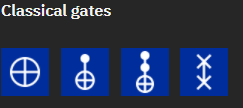
\includegraphics[width=\textwidth]{img/classical-gates.PNG}
        \caption{A visual representation of the classical gates}
        \label{fig:classical gates}
\end{figure}

\begin{table}[]
\label{tab:pgates}
        \begin{tabular}{l|l}
        \hline
        \multicolumn{1}{|l|}{Phase Gate}  & \multicolumn{1}{l|}{Matrix representation of the gate}               \\ \hline
        T                                 & $\begin{pmatrix}1&0 \\ 0& \exp(i\frac{\theta}{4})\end{pmatrix}$      \\
        Z                                 & $\begin{pmatrix}1&0 \\ 0& -1\end{pmatrix}$                           \\
        S                                 & $\begin{pmatrix}1&0 \\ 0& i\end{pmatrix}$                            \\
        T$\dagger$                        & $\begin{pmatrix}1&0 \\ 0& \exp(-i\frac{\theta}{4})\end{pmatrix}$     \\
        S$\dagger $                       & $\begin{pmatrix}1&0 \\ 0& -i\end{pmatrix}$                           \\
        P                                 & $\begin{pmatrix}1&0 \\ 0& \exp(i\lambda)\end{pmatrix}$               \\
        RZ                                & $\begin{pmatrix}\exp(-i\frac{\lambda}{2})&0 \\ 0& \exp(i\frac{\lambda}{2})\end{pmatrix}$                                    
        \end{tabular}
        \caption{Matrix representations of the phase gates.}
\end{table}
    
\begin{figure} [h]
    \centering
    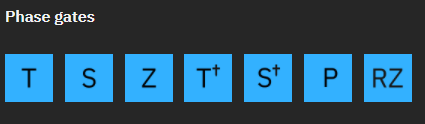
\includegraphics[width=\textwidth]{img/phase-gates.PNG}
        \caption{A visual representation of the phase gates}
        \label{fig:phase gates}
\end{figure}

\begin{figure} [h]
    \centering
    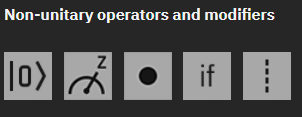
\includegraphics[width=\textwidth]{img/non-unitary-gates.PNG}
        \caption{A visual representation of the non-unitary gates}
        \label{fig:non-uni gates}
\end{figure}

\begin{figure} [h]
    \centering
    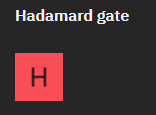
\includegraphics[width=\textwidth]{img/hadamard-gate.PNG}
        \caption{A visual representation of the hadamard gate}
        \label{fig:hadamard gates}
\end{figure}

\begin{table}[]
\label{tab:qgates}
        \begin{tabular}{l|l}
        \hline
        \multicolumn{1}{|l|}{Phase Gate}  & \multicolumn{1}{l|}{Matrix representation of the gate}                                                                                                                                                                                                                         \\ \hline
        RX                                & $\begin{pmatrix} \cos\frac{\theta}{2}&-i\sin\frac{\theta}{2}              \\ -i\sin\frac{\theta}{2}&\cos\frac{\theta}{2}                                                                                                                                        \end{pmatrix}$ \\
        RY                                & $\begin{pmatrix} \cos\frac{\theta}{2}&-\sin\frac{\theta}{2}               \\ \cos\frac{\theta}{2}&\sin\frac{\theta}{2}                                                                                                                                          \end{pmatrix}$ \\
        RXX                               & $\begin{pmatrix} \cos\frac{\theta}{2}&0&0&-i\sin\frac{\theta}{2}          \\ 0&\cos\frac{\theta}{2}&-i\sin\frac{\theta}{2}&0                           \\ 0&-i\sin\frac{\theta}{2}&\cos\frac{\theta}{2}&0 \\ -i\sin\frac{\theta}{2}&0&0&\cos\frac{\theta}{2}    \end{pmatrix}$ \\                               
        RZZ                               & $\begin{pmatrix} \exp(-i\frac{\theta}{2})&0&0&0                           \\ 0&\exp(i\frac{\theta}{2})&0&0                                             \\ 0&0&\exp(i\frac{\theta}{2})&0 \\ 0&0&0&\exp(-i\frac{\theta}{2})                                       \end{pmatrix}$ \\         
        $\sqrt{X}$                        & $\begin{pmatrix} 1+i&1-i                                                  \\ 1-i&1+i                                                                                                                                                                            \end{pmatrix}$ \\
        $\sqrt{X}\dagger$                 & $\begin{pmatrix} 1-i&1+i                                                  \\ 1+i&1-i                                                                                                                                                                            \end{pmatrix}$ \\
        U                                 & $\begin{pmatrix} \cos\frac{\theta}{2}&-\exp(i\lambda)\sin\frac{\theta}{2} \\ \exp(i\phi)\sin\frac{\theta}{2}&\exp(i(\phi+\lambda))\cos\frac{\theta}{@}                                                                                                          \end{pmatrix}$ \\
        Y                                 & $\begin{pmatrix} 0&-i \\ i&0                                                                                                                                                                                                                                    \end{pmatrix}$                                   
        \end{tabular}
        \caption{Matrix representations of the quantum gates.}
\end{table}

\begin{figure} [h]
    \centering
    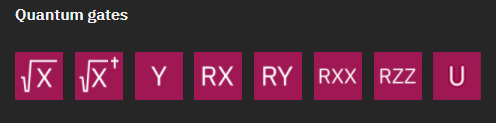
\includegraphics[width=\textwidth]{img/quantum-gates.PNG}
        \caption{A visual representation of the quantum gates}
        \label{fig:quantum gates}
\end{figure}

\subsubsection{The algorithm}

Shor's algorithm is already build for anybody to use in Qiskit \footnote{Qiskit is the open source SDK from IBM for working with OpenQasm}. There is documentation written with the code fo further explaination.
The code is run in IBM's Quantum lab, but the circuit is also available on the composer. Since it would be useless to rewrite the algorithm, this study will use this code and run it in Quantum Lab.


\section{Other algorithms}
\label{sec:Other algorithms}
\section{The use of quantum computing}